\documentclass[10pt,a4paper]{article}
\usepackage[margin=23mm]{geometry}
\usepackage[T1]{fontenc}
\usepackage{lmodern,microtype,amsmath,amssymb,booktabs,graphicx,float}
\usepackage[small,bf]{caption}
\usepackage{xcolor}
\usepackage{tikz}
\usetikzlibrary{arrows.meta,positioning}
\usepackage[colorlinks=true,linkcolor=teal,urlcolor=teal,citecolor=teal]{hyperref}
\newcommand{\rpc}[1]{\mbox{\texttt{#1}}}
\setlength{\parskip}{4pt}
\setlength{\parindent}{0pt}
\setlength{\emergencystretch}{2em}
% Generated from actual observations; do not edit.
\newcommand{\FaultCount}{10,000}
\newcommand{\CheckCount}{3,774,447}
\newcommand{\ElectionCount}{603}
\newcommand{\ChangeCount}{469}
\newcommand{\CommittedCount}{1,570}
\newcommand{\EntryCount}{2,170}
\newcommand{\ClientSuccess}{1,516}
\newcommand{\ClientRejected}{2,576}
\newcommand{\ClientTimeout}{167}
\newcommand{\LatencyTrials}{100}
\newcommand{\ElectionTrials}{200}
\newcommand{\RecoveryTrials}{20}
\newcommand{\WritesPerTrial}{5}
\newcommand{\OfferedPerLoss}{500}
\newcommand{\TotalLossAttempts}{4,500}
\newcommand{\BootstrapReplicates}{2,000}
\newcommand{\SimulationSeconds}{574.22}
\newcommand{\CampaignWallSeconds}{86.57}
\newcommand{\LatencySeedRange}{10000--10099}
\newcommand{\ElectionSeedRange}{20000--20199}
\newcommand{\RecoverySeedRange}{30000--30019}
\newcommand{\LatencyRows}{%
0 & 8.03 & 12.03 & 13.88 & 500/500 & 0 & 0 \\
10 & 8.78 & 14.60 & 18.42 & 500/500 & 0 & 0 \\
20 & 9.61 & 18.07 & 26.02 & 500/500 & 0 & 0 \\
30 & 11.25 & 64.40 & 119.64 & 500/500 & 0 & 0 \\
40 & 13.21 & 116.39 & 263.81 & 500/500 & 0 & 0 \\
50 & 23.27 & 259.41 & 800.70 & 498/500 & 2 & 0 \\
60 & 67.54 & 1132.76 & 2208.73 & 487/500 & 9 & 4 \\
70 & 120.94 & 2298.28 & 2823.63 & 391/500 & 92 & 17 \\
80 & 169.34 & 2607.67 & 2900.48 & 128/500 & 179 & 193 \\
}
\newcommand{\UncertaintyRows}{%
0 & {[}7.68, 8.28{]} & {[}11.71, 12.57{]} & {[}13.01, 14.80{]} & {[}100.00, 100.00{]} \\
10 & {[}8.35, 9.24{]} & {[}13.66, 15.16{]} & {[}16.10, 19.71{]} & {[}100.00, 100.00{]} \\
20 & {[}9.14, 10.17{]} & {[}15.82, 19.51{]} & {[}21.83, 63.22{]} & {[}100.00, 100.00{]} \\
30 & {[}10.62, 11.79{]} & {[}59.38, 66.78{]} & {[}77.52, 167.84{]} & {[}100.00, 100.00{]} \\
40 & {[}12.53, 14.14{]} & {[}112.77, 162.59{]} & {[}174.72, 429.24{]} & {[}100.00, 100.00{]} \\
50 & {[}18.38, 57.23{]} & {[}213.01, 310.90{]} & {[}508.34, 1601.09{]} & {[}99.00, 100.00{]} \\
60 & {[}64.06, 107.46{]} & {[}905.57, 1494.00{]} & {[}1886.38, 2513.82{]} & {[}95.40, 99.00{]} \\
70 & {[}115.35, 168.79{]} & {[}2136.08, 2515.40{]} & {[}2674.46, 2878.04{]} & {[}74.00, 82.40{]} \\
80 & {[}117.20, 210.44{]} & {[}2357.12, 2864.63{]} & {[}2631.07, 2977.12{]} & {[}20.60, 30.40{]} \\
}
\newcommand{\ElectionRows}{%
3 & Initial & 197.48 & 263.57 & 1.075 & 8.66 & 0 & 0.0 \\
3 & Recovery & 212.72 & 454.49 & 1.220 & 6.66 & 22 & 10.0 \\
5 & Initial & 190.60 & 236.41 & 1.190 & 18.34 & 1 & 0.5 \\
5 & Recovery & 195.33 & 330.23 & 1.225 & 15.95 & 11 & 5.5 \\
}
\newcommand{\RecoveryRows}{%
Leader crash & 195.57 & 237.83 & 0 \\
Minority partition & 201.43 & 283.68 & 0 \\
Partition healing & 60.31 & 64.08 & 0 \\
Outdated follower restart & 8.39 & 9.97 & 0 \\
}
\newcommand{\AbstractFindings}{At 80\% packet loss, 128 of 500 offered attempts committed, compared with 500 of 500 at zero loss. Initial median election convergence was 197\,ms for three nodes and 191\,ms for five nodes under the stated network model.}
\newcommand{\LatencyFindings}{From 0\% to 20\% packet loss, all 500 writes committed at each loss rate, with p95 latency remaining below 19\,ms (18.07\,ms at 20\% loss) and p99 beginning to reflect retry delays (26.02\,ms, 95\% CI {[}21.83, 63.22{]}\,ms). Because a three-node leader needs confirmation from only one of its two followers, a proposal commits in one round trip whenever at least one follower's request--response pair survives. Under independent 20\% per-packet loss on both requests and responses, both followers fail the initial round trip with probability $(1 - 0.8^2)^2 = 12.96\%$ (67 of 500 attempts in this run). Although \texttt{propose()} resets the 50\,ms heartbeat deadline, each seed submits five back-to-back writes as soon as the faster follower commits the prior entry; delayed acknowledgements from the slower follower and from commit-advance broadcasts remain in flight and trigger immediate follow-up \rpc{AppendEntries} batches whenever \texttt{next\_index} lags the leader's log, recovering 63 of those 67 dual-drop writes in under 50\,ms. By 30\% loss, compound drops across both followers routinely sever this pipelined recovery and stall until the 50\,ms periodic heartbeat, pushing p95 to 64.40\,ms and p99 to 119.64\,ms. \par Above 50\% loss, dropped heartbeats and vote traffic also trigger follower election timeouts and split elections, dominating tail latency and availability. At 80\% loss, only 128 of 500 attempts commit, with successful-write p95 reaching 2,607.67\,ms; 179 attempts time out and 193 find no leader. Figure~\ref{fig:latency} pairs latency with outcome proportions because failed attempts contribute no successful-latency sample.}
\newcommand{\ElectionFindings}{All 800 election phases across 400 cluster trials converged within the three-second deadline. Five-node startup was slightly faster at the median than three-node startup (190.60 versus 197.48\,ms), consistent with the earlier minimum of five independent election timers, while sending roughly twice as many RPCs (18.34 versus 8.66) to win a quorum and notify every live peer. \par In Table~\ref{tab:elections}, ``Attempts'' counts total candidate transitions across the cluster before convergence, whereas ``Split terms'' counts terms in which multiple candidacies prevented any node from winning a majority. During three-node initial startup, 7.5\% of trials (15/200) saw a second node become a candidate before the first candidate's \rpc{RequestVote} arrived (1.075 mean attempts), yet the split-term rate was 0.0\% because the third undecided voter broke every tie. After a three-node leader crash, however, only two live voters remain: if both time out in the same term and vote for themselves, neither can reach a quorum of two. Consequently, split votes occurred in 10.0\% of three-node recovery trials (20/200 trials, 22 split terms) versus 5.5\% for five-node recovery (11/200 trials, 11 split terms).}
\newcommand{\RecoveryFindings}{All 80 scenario trials recovered within their deadlines.}
\newcommand{\OutdatedMedian}{8.39}
\newcommand{\OutdatedNinetyFive}{9.97}
\newcommand{\TCPFindings}{A separate localhost benchmark sent 100 sequential writes through three independent Python processes (startup and initial election excluded), each backed by \texttt{FileStorage} on Windows 11 (NTFS). All 100 writes committed and were applied by every node; client-visible median latency was 15.96\,ms and p95 was 30.45\,ms, compared with the no-loss simulator median of 8.03\,ms. The ${\approx}7.9$~ms median premium over the no-loss simulator (15.96\,ms vs.\ 8.03\,ms) reflects the combined cost of sequential NTFS \texttt{os.fsync} and atomic file-replacement operations (on the leader and first acknowledging follower), loopback TCP framing, and client-reply delivery.}
\newcommand{\SensitivityFindings}{All five mutants triggered a recorded assertion, and all five correct controls completed without a safety violation.}
\newcommand{\SensitivityRows}{%
\texttt{NoElectionRestriction} & Omit candidate log-freshness restriction & Leader Completeness \\
\texttt{DoubleVote} & Grant a fresh candidate a second vote in the same term & Persisted-vote consistency \\
\texttt{ForgetVoteOnRestart} & Acknowledge an external vote without its durable write & Durable/volatile state agreement \\
\texttt{NaiveCommit} & Count an older-term replicated quorum without a current-term entry & Leader Completeness \\
\texttt{CommitBeyondMatch} & Cap follower commitment by local log end instead of the RPC-verified prefix & Committed-entry agreement \\
}

\title{RaftLight: Crash-Fault Consensus, Adversarial Testing,\\and Reproducible Simulation}
\author{RaftLight Project\\\small Stage 1 engineering evaluation}
\date{24 October 2026}

\begin{document}
\maketitle
\begin{abstract}
Consensus lets independently failing servers maintain an ordered replicated state
machine. RaftLight implements fixed-membership Raft for three or five Python
nodes, with durable term, vote and log state, asynchronous localhost RPCs, and a
deterministic network simulator exercising the same consensus engine. Targeted
tests, Hypothesis event sequences, and a campaign of \FaultCount{} chaos actions
(faults, repairs and parser checks) check historical election, log, commitment and application
properties. The campaign observed no safety violations in \CheckCount{} property
group checks; all twenty runs converged after stable connectivity and restarts.
\AbstractFindings{}
\end{abstract}

\section{Introduction}
A replicated state machine executes the same deterministic operations in the
same order on multiple servers~\cite{schneider}. The difficult part is agreeing on that order when
servers stop, packets disappear, and different machines observe events at
different times. Raft decomposes this problem into leader election, log
replication, and safety restrictions~\cite{raft}. A leader orders client writes;
a majority establishes which entries can survive subsequent leadership changes.
Paxos established a foundational quorum-based approach to this problem~\cite{lamport};
Raft organizes similar safety obligations around a strong leader and explicit
election restrictions.

RaftLight connects these protocol rules to executable counterexample searches
and reproducible measurements. It implements the standard election and
replication rules, including the current-term commitment restriction. It includes
neither membership changes nor log compaction. Its key-value workload supports
\texttt{SET} and \texttt{DELETE}; leader no-ops provide a current-term commitment
point after election.

Safety and liveness require separate evidence. Safety excludes conflicting
decisions even while a cluster is partitioned. Liveness means eventual progress
under conditions that permit a majority to communicate. An isolated old leader
may retain its role while a majority elects a leader in a higher term. Such
different-term coexistence is expected; successful minority commitment would be
a violation. Tests therefore preserve history and separately exercise recovery
under stable conditions.

\section{System model and architecture}
Membership is fixed at $N\in\{3,5\}$. Servers have unique integer identifiers and
exchange asynchronous \rpc{RequestVote} and \rpc{AppendEntries} requests and responses.
Messages may be lost, duplicated, delayed, reordered, or prevented by directional
connectivity. Servers fail by stopping and restart from durable state. Peers are
trusted to execute the protocol; input validation rejects malformed requests.

A quorum has size
\[
q = \lfloor N / 2 \rfloor + 1.
\]
Two quorums intersect because $2q > N$. A later election therefore includes at
least one server from the majority that stored a committed entry. Preserving
that entry also depends on the election freshness restriction and current-term
commitment rule.

\begin{figure}[htbp]\centering
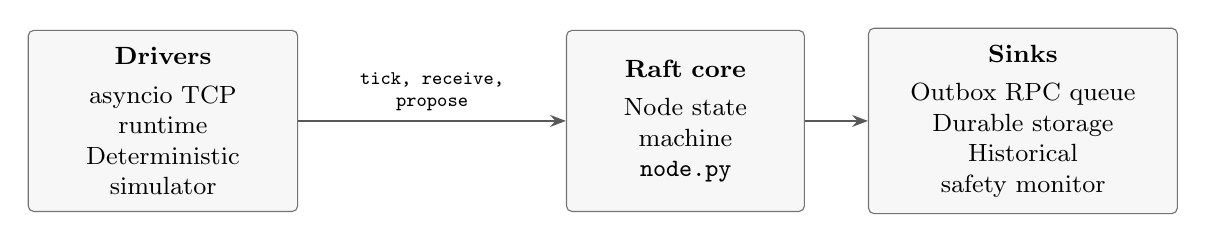
\begin{tikzpicture}[
  block/.style={draw=black!55,rounded corners=2pt,fill=black!3,
    align=center,minimum height=23mm,font=\small,inner sep=6pt},
  flow/.style={-{Stealth[length=2mm]},thick,draw=black!65}]
\node[block,text width=30mm] (drivers) {\textbf{Drivers}\\[3pt]
  asyncio TCP runtime\\Deterministic simulator};
\node[block,text width=26mm,right=34mm of drivers] (core) {
  \textbf{Raft core}\\[3pt]Node state machine\\\texttt{node.py}};
\node[block,text width=35mm,right=8mm of core] (sinks) {\textbf{Sinks}\\[3pt]
  Outbox RPC queue\\Durable storage\\Historical safety monitor};
\draw[flow] (drivers.east) -- node[above,align=center,font=\scriptsize]
  {\texttt{tick, receive,}\\\texttt{propose}} (core.west);
\draw[flow] (core.east) -- (sinks.west);
\end{tikzpicture}
\caption{The Sans-I/O boundary separates scheduling and transport from consensus.
The \texttt{storage.py} abstraction provides durable state; observer events feed
the historical safety monitor.}
\end{figure}

The same \texttt{Node} state machine drives both execution environments.
Its caller serializes \texttt{tick}, \texttt{receive}, and \texttt{propose}, so
the consensus code performs no socket operations or sleeps. The \texttt{asyncio}
TCP runtime supplies monotonic wall-clock time and independent outgoing peer
queues; the simulator controls virtual time and packet delivery. Tests therefore
exercise the consensus implementation used by the TCP runtime.

\subsection{Durable and volatile state}
Each server durably stores its current term, vote, and complete log. Index zero
is a permanent dummy no-op with term zero; real entries begin at one. Terms in a
valid log are nondecreasing. The commit index, application position, role, timer
deadlines and leader replication maps are volatile.

While the simulator preserves immutable snapshots in memory across node
restarts, the TCP runtime persists each term, vote or log change to disk.
\texttt{storage.py} writes a full JSON snapshot to a sibling temporary file,
flushes it, calls \texttt{os.fsync} and atomically replaces the previous snapshot.
POSIX systems also synchronize the parent directory; Windows omits that step
because Python has no portable directory-sync API. Corrupt snapshots prevent
startup, preserving prior votes and log entries from an accidental reset.
Each state file has one owner, and durability assumes reliable local flush and
replace semantics; sudden host power loss is not tested.

A node persists state before sending any acknowledgement that depends on it.
If storage fails, that instance stops permanently; restarting constructs a new
node from the durable snapshot. Because commit and application indexes are
volatile, the restarted node waits to learn which prefix is committed before
replaying it. A newly elected leader appends a no-op, allowing earlier entries
to become committed without waiting for another client write.

\section{Consensus implementation}
\subsection{Election and term handling}
Followers and candidates independently choose election deadlines in
150--300\,ms, while leaders send heartbeats every 50\,ms. When a deadline expires,
the candidate increments its term, persists its self-vote and sends
\rpc{RequestVote} RPCs. It becomes leader once a majority has voted for it, counting each
voter only once. If the election splits, a fresh randomized deadline starts
another attempt.

A voter compares $(t_{\mathrm{last}}, i_{\mathrm{last}})$ lexicographically:
last term takes priority over length. For candidate $c$ and voter $v$,
\begin{equation}
\begin{aligned}
\mathrm{fresh}(c, v) \iff{}& t_{\mathrm{last}}(c) > t_{\mathrm{last}}(v)\\
&{}\lor\bigl(t_{\mathrm{last}}(c) = t_{\mathrm{last}}(v)
\land i_{\mathrm{last}}(c) \geq i_{\mathrm{last}}(v)\bigr).
\end{aligned}
\end{equation}
A voter grants a request only when the candidate's log is at least as current
as its own and it has not voted for another candidate in that term. After
validating the message and its sender, the receiver persists any higher term,
clears its previous vote and becomes a follower before handling the RPC.
Same-term \rpc{AppendEntries} also makes a candidate step down, whereas lower-term
leader traffic cannot postpone an election.

\subsection{Replication and commitment}
When a leader receives a proposal, it appends and persists the entry before
sending \rpc{AppendEntries} batches of up to eight entries. It tracks each follower
through \texttt{next\_index} and \texttt{match\_index}. A follower rejects a
request whose preceding index and term do not match its log, returning either
the first missing index or the conflicting term and its first index. The leader
can then skip a conflicting term while backtracking. Bounding each
\rpc{AppendEntries} batch to eight entries caps per-message serialization work
while still allowing moderate follower backlogs (such as the eight-write outage
in Section~\ref{sec:recovery}) to recover in a single batch; the transport
layer independently bounds wire frame size.

Once the preceding entry matches, the follower retains the matching prefix and
replaces its suffix only at an actual conflict. A short duplicate request
therefore cannot erase a longer matching suffix. It advances commitment only
through the prefix verified by that request, preventing a delayed heartbeat from
committing unrelated trailing entries. Committed entries are applied sequentially
to the in-memory key-value store, where \texttt{DELETE} is idempotent on missing keys.

For a leader, advancement to index $k$ requires
\[
k > \mathrm{commitIndex},\qquad
\Bigl\lvert\{s : \mathrm{matchIndex}_s \geq k\}\Bigr\rvert \geq q,\qquad
\mathrm{log}[k].\mathrm{term} = \mathrm{currentTerm}.
\]
The leader counts its own copy toward the quorum. Once an entry from its current
term commits, every preceding entry commits with it. Replication on a majority
alone cannot directly commit an earlier-term entry; the regression based on
Figure~8 of the Raft paper~\cite{raft} exercises this case.

Request identifiers bind each replication response to the request that produced
it. A delayed rejection cannot reverse newer progress, repeated responses have
no additional effect, and an acknowledgement can cover only the entries sent
in its request.

\subsection{Runtime and client semantics}
Each runtime listens independently over \texttt{asyncio} TCP and maintains a
bounded outgoing queue for every peer. Requests are bounded, newline-delimited
JSON frames. Because each peer has its own sender, a failed follower cannot hold
up communication with the others. Startup, shutdown and fatal background errors
have explicit handling. Testing these runtime boundaries alongside the protocol
follows the engineering concerns described in \emph{Paxos Made Live}~\cite{paxoslive}.

A runtime review exposed a failure at the storage--transport boundary: a
persistence error could enter the ordinary network-error path. Such errors now
latch a fatal state, preventing a connection retry from resuming a node whose
durable state is uncertain.

Because appending a proposal does not establish commitment, \texttt{propose()}
returns its assigned log index. The TCP adapter retains the exact entry at that
position and acknowledges the client only after commitment and application.
If leadership changes or the request times out, the outcome remains unknown:
another leader may subsequently commit the command, and retries have no
client-session deduplication guarantee. Status reads expose local state and a
leader hint, so they may be stale.

\section{Safety properties and executable checks}
The protocol's established reasoning~\cite{raft} motivates the implementation
and the following executable predicates. Let $L_s(\tau)$ denote node $s$'s log
at time $\tau$, with each entry containing a term and command. Let $E(t)$ be the
set of node identities elected in term $t$. Histories retain events across crashes.

\textbf{Election Safety.} At most one node may be elected in a term. Durable
single voting and intersecting majorities support this property. The monitor
records every leadership event by term, including leaders that later crash or
step down.
\begin{equation}
\forall t:\quad |E(t)| \leq 1.
\end{equation}

\textbf{Log Matching.} If two nodes have entries with the same index and term,
their entire prefixes through that index must agree, including commands. The
monitor compares complete prefixes, including durable logs of crashed nodes.
Consistent \rpc{AppendEntries} prefix checks and leader append-only behavior support
this property.
\begin{equation}
\begin{aligned}
\forall s,r,i,\tau:\quad
L_s(\tau)[i].\mathrm{term} = L_r(\tau)[i].\mathrm{term}
\ \Longrightarrow\ \\
L_s(\tau)[1{:}i] = L_r(\tau)[1{:}i],
\end{aligned}
\end{equation}
where $i$ exists in both logs and $[1{:}i]$ includes index $i$.

\textbf{Leader Completeness.} A committed entry must occur in every leader
elected in a subsequent term. Historical election snapshots are compared with
committed entries and their leader commitment terms. Checks run both at election
and when an older commitment is first observed, so delayed observations do not
erase the obligation. The freshness rule and current-term commitment condition
are the critical mechanisms.
\begin{equation}
\begin{aligned}
\mathrm{Commit}(i, e, t) \land u > t \land \mathrm{Elected}(s, u)
\ \Longrightarrow\ \\
L_s\bigl(\tau_{\mathrm{election}}(s,\, u)\bigr)[i] = e.
\end{aligned}
\end{equation}
Here $\mathrm{Commit}(i, e, t)$ means a leader commits entry $e$ at index $i$
while in term $t$; $e$ may have been appended in an earlier term.
The time $\tau_{\mathrm{election}}(s,\, u)$ is when node $s$ is elected in term $u$.

\textbf{State Machine Safety.} No two applications at the same index may contain
different entries. A global application history survives restarts and is checked
against each local committed prefix. The expected key-value map is rebuilt from
that prefix and compared with the node's map.
\begin{equation}
\mathrm{Apply}(s, i, e, \tau) \land
\mathrm{Apply}(r, i, e', \tau') \ \Longrightarrow\ e = e'.
\end{equation}

Additional checks cover nondecreasing durable terms, consistent same-term votes,
durable/in-memory agreement,
$0 \leq \mathrm{lastApplied} \leq \mathrm{commitIndex} < \lvert\mathrm{log}\rvert$,
valid leader replication indexes, and no processing by crashed
nodes. Per-node committed prefixes must survive restart, and commit/application
positions may reset only in a new node incarnation. The cumulative check count
covers evaluations of all nine invariant groups after internal deliveries,
timer transitions and injected actions.

\subsection{Oracle sensitivity via protocol mutation}
Five isolated mutants each remove one protocol safeguard while retaining the
production message and state-transition interfaces. Deterministic witnesses run
the altered code and the historical safety monitor, then repeat the same schedule
with the correct Node as a control. The table records the monitor's first
assertion for each witness.
\SensitivityFindings{}

\begin{table}[H]\centering\footnotesize
\caption{Executed mutant witnesses. Each correct implementation control passes.
The final column names the first assertion actually raised.}
\setlength{\tabcolsep}{4pt}
\begin{tabular}{p{.22\linewidth}p{.39\linewidth}p{.31\linewidth}}\toprule
Mutant & Injected defect & First detected invariant\\\midrule
\SensitivityRows
\bottomrule\end{tabular}
\end{table}

The paired traces and detection messages are saved in
\path{results/sensitivity_summary.json}. The mutation witnesses exercise the
oracle separately from the unmodified-engine chaos campaign.
The double-vote witness uses a plain snapshot store in both arms to expose the
monitor; production storage independently rejects a changed same-term vote.
The missing-vote mutant is detected at its first durable/volatile disagreement;
a separate recorded continuation exercises crash, restart and a second vote.
The commit-cap witness starts both arms at an explicitly initialized conservative
retry cursor, then uses the production sender for its eight-entry batch.

\section{Adversarial testing methodology}
\subsection{Generated and targeted scenarios}
Hypothesis \mbox{\texttt{RuleBasedStateMachine}}~\cite{hypothesis} generates event sequences over
both cluster sizes. Actions advance time; deliver, drop, duplicate and delay
messages; alter symmetric or asymmetric connectivity; crash and restart nodes;
set packet loss; submit writes; and provoke simultaneous elections. The saved
configuration uses eighty generated examples with seventy steps per example,
deterministic generation, no real sleeps, and shrinking on failure. Every
completed sequence has a stable recovery phase.

Targeted tests complement the generated schedules at specific protocol
boundaries. The Raft Figure~8 regression checks that counting replicas alone
cannot commit an older-term entry, while replication tests exercise conflicting
suffixes, delayed responses and short duplicate appends. Storage tests inject
replacement failures and reject corrupted snapshots; real TCP tests cover
three- and five-node failover, restart and minority write timeouts.

\subsection{The 10,000-event campaign}
Twenty independent runs alternate between three and five nodes, using seeds
20261022 through 20261041 and 500 counted events per run. An eleven-way random
selector chooses node crashes, restarts, packet drops, delays, duplicates,
symmetric partitions, partition healing, directional link changes, stale RPC
delivery, message reordering, and malformed-input checks. When a node crash is
selected, the trace records the victim's role at the instant of failure
(follower, leader, or candidate), expanding the eleven selector branches into
the thirteen action categories shown in Figure~\ref{fig:chaos}
($688 + 475 + 277 = 1{,}440$ total crashes). A selection counts only when its
preconditions hold. The 10,000-action budget covers injected faults, effective
repairs and parser checks; ordinary ticks and periodically offered client writes
continue between injections without using that budget.

The campaign offers a unique-valued SET every four scheduling cycles, recording
commitments within a 0.75~s simulated deadline separately from rejections and
timeouts. Every sixty cycles it attempts network repair and node restarts to
allow intermittent progress. After the 500 counted events, a separate recovery
phase restarts every crashed node, restores reliable connectivity and requires
full convergence within five simulated seconds.

The event trace, client outcomes, final state, and recent RPC history are saved
for every run. On an invariant failure the runner writes the full available
snapshot before propagating the failure. Reproduction uses the recorded seed,
cluster-size schedule, campaign arguments, Python version and source revision.
Hypothesis supplies a shrunk action sequence and diagnostic JSON on failure.

\section{Experimental evaluation}
\subsection{Common conditions}
All plotted latency and recovery values use simulated time. Delays are independent
uniform samples between 1 and 10\,ms. Timers are polled at 5\,ms resolution. Packet
loss applies independently to each sent request and response, including election
traffic. Simulation excludes serialization cost, disk delay, CPU scheduling and
client-network round trips. Raw observations are in
\texttt{results/benchmark\_raw.json}; summary statistics and configuration are in
\texttt{results/benchmark\_summary.json}.

Loss trials use \LatencyTrials{} seeds (\LatencySeedRange{}), election trials use
\ElectionTrials{} seeds per size (\ElectionSeedRange{}), and recovery trials use
\RecoveryTrials{} seeds per scenario (\RecoverySeedRange{}). Quantiles use
NumPy's linear percentile estimator. Confidence intervals resample entire seed
blocks, preserving dependence among the offered operations within a trial;
\BootstrapReplicates{} bootstrap replicates give the 2.5th and 97.5th percentiles.
The supplementary table reports these intervals for latency and availability.

\subsection{A: packet loss and commit latency}
Three-node clusters offer \WritesPerTrial{} sequential SET attempts per seed at each loss
rate: \OfferedPerLoss{} attempts per condition, \TotalLossAttempts{} total. Startup permits five simulated
seconds for election, and between attempts permits one second for leader
discovery. Each accepted proposal has a three-second commit deadline. The
measurement ends at the first observed commitment of that exact command, even
if leadership changes. No-leader and timeout outcomes remain in the success
denominator and are excluded from successful-latency quantiles.

\begin{table}[H]\centering\small
\caption{Packet loss experiment. Latency units are simulated milliseconds.}
\label{tab:loss}
\begin{tabular}{rrrrrrr}\toprule
Loss (\%) & p50 & p95 & p99 & Committed & Timeout & No leader\\\midrule
\LatencyRows
\bottomrule\end{tabular}
\end{table}
\begin{figure}[H]\centering
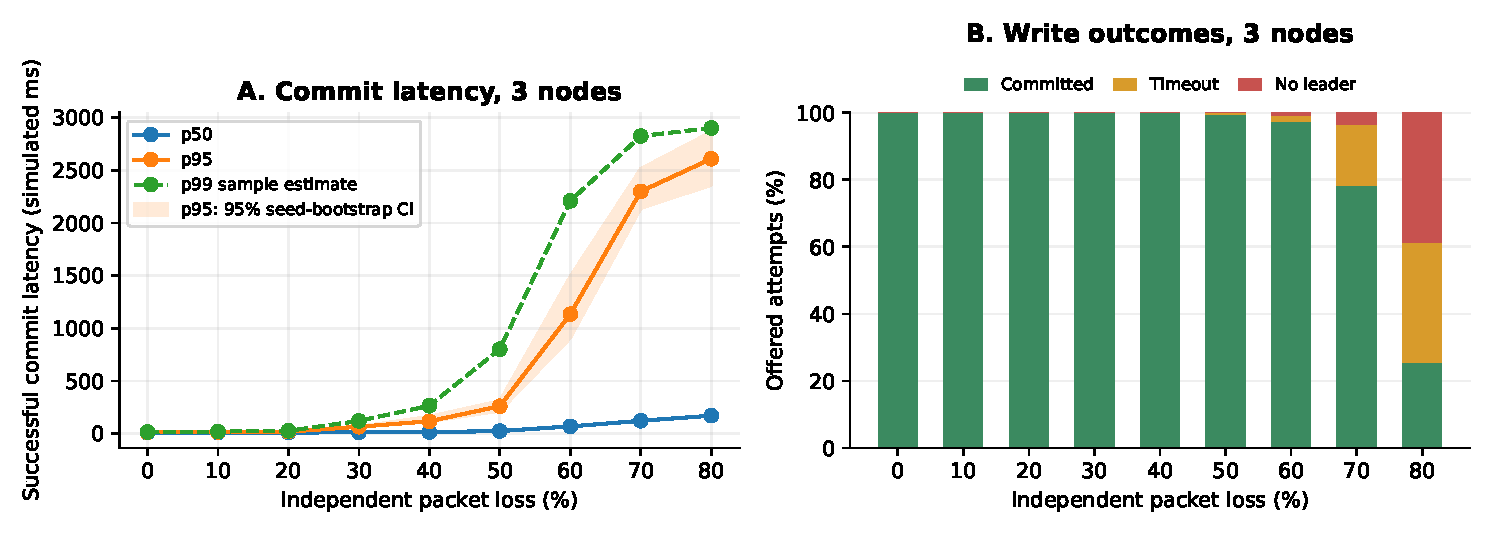
\includegraphics[width=\linewidth]{figures/latency_vs_packet_loss.pdf}
\caption{Commit latency among successful attempts (A) and the proportions of
committed, timed-out and no-leader attempts (B).}
\label{fig:latency}
\end{figure}

\LatencyFindings{}

\subsection{B: cluster size and election convergence}
Convergence means every live node recognizes the highest-term leader. Initial
convergence begins at time zero; failure recovery begins when the leader crashes
after the initial no-op has converged. Each phase has a three-second deadline.
RPC counts include requests, responses and sends addressed to stopped nodes.
A split-vote term is a term with multiple observed candidacies and no elected
leader by the end of the measurement.

\begin{table}[H]\centering\small
\caption{\ElectionTrials{} seeds per size. Attempts and RPCs are means;
latencies are simulated ms. Split rate is the percentage of trials with a split term.}
\label{tab:elections}
\begin{tabular}{rlrrrrrr}\toprule
Nodes & Phase & p50 & p95 & Attempts & RPCs & Split terms & Split (\%)\\\midrule
\ElectionRows
\bottomrule\end{tabular}
\end{table}
\begin{figure}[H]\centering
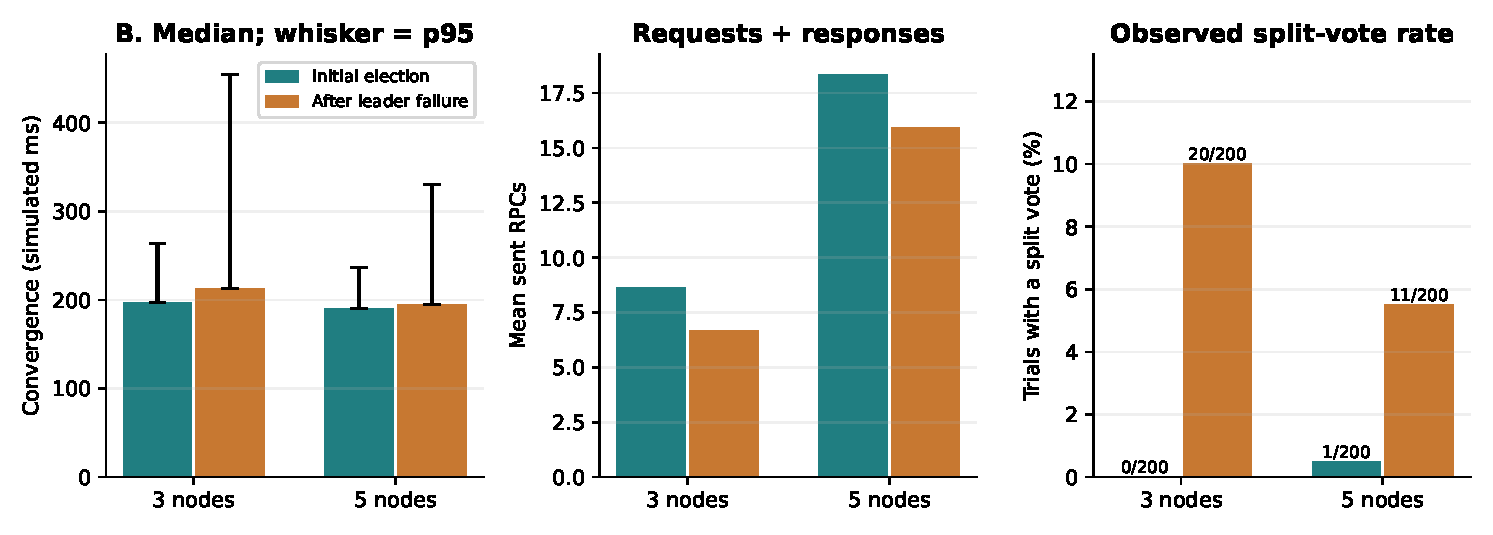
\includegraphics[width=\linewidth]{figures/election_convergence.pdf}
\caption{Election convergence, message cost and observed split-vote trial rates.}
\label{fig:elections}
\end{figure}

\ElectionFindings{}

This 10.0\% three-node recovery split rate follows directly from the simulator's
timing model. Although the 150\,ms election timeout window spans thirty 5\,ms
polling ticks (giving a $1/30 \approx 3.3\%$ chance of two independent timers
expiring on the exact same tick from a common reference), a split vote occurs
whenever the second follower's deadline expires before the first candidate's
\rpc{RequestVote} arrives over the 1--10\,ms network link, compounded by
1--10\,ms differential arrival times of the crashed leader's final heartbeat.
Because that vulnerability window spans roughly $\pm 1$ to $2$ polling ticks
around the first candidate's wakeup (two to three ticks out of thirty), the
expected collision rate rises from 3.3\% into the 7--10\% range, matching the
observed 10.0\% trial rate.

\subsection{C: recovery scenarios}
\label{sec:recovery}
Each scenario uses five nodes and \RecoveryTrials{} seeds. Leader-crash and
minority-partition scenarios measure write availability, so they end as soon as
the surviving majority commits a new entry. The minority partition contains the
old leader and one follower, leaving the other three to elect a leader. Healing
and outdated-follower restart measure full convergence: they continue until all
five logs, commit indexes and state machines agree. The outdated follower misses
eight SET commands before restarting.

\begin{table}[H]\centering\small
\caption{Five-node recovery, simulated ms; \RecoveryTrials{} trials per scenario.}
\begin{tabular}{lrrr}\toprule
Scenario & p50 & p95 & Timeouts\\\midrule
\RecoveryRows
\bottomrule\end{tabular}
\end{table}
\begin{figure}[H]\centering
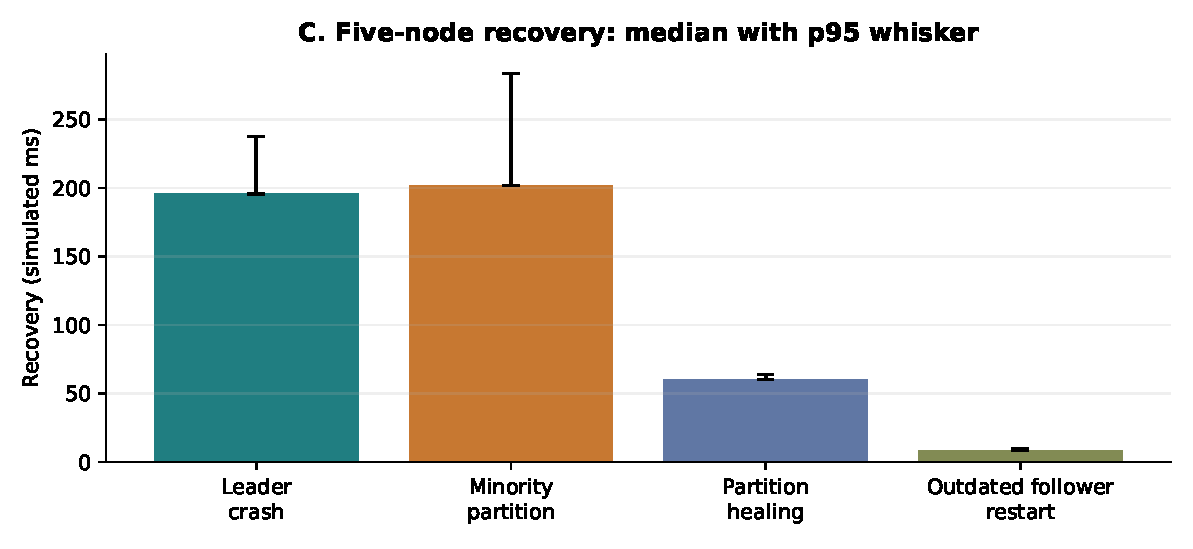
\includegraphics[width=.94\linewidth]{figures/recovery_performance.pdf}
\caption{Five-node recovery: time to a new majority write after leader crash or
minority partition, and time to full convergence after healing or follower restart.}
\end{figure}

\RecoveryFindings{}
Leader replacement took roughly one election timeout, while partition healing
took one heartbeat interval plus message delivery. Because the eight missed
commands fit inside a single eight-entry \rpc{AppendEntries} batch, catch-up
requires no multi-round backtracking: when the eighth write commits right before
restart, the leader's commit-notification \rpc{AppendEntries} already in transit
on the 1--10\,ms link (or the next scheduled heartbeat) delivers the missing
suffix and commit index together, yielding the \OutdatedMedian{}\,ms median
(p95: \OutdatedNinetyFive{}\,ms) across all five nodes.

\subsection{D: campaign observations}
The campaign observed \ElectionCount{} successful elections and \ChangeCount{}
changes of leader identity between consecutive leadership events. Across the
twenty runs, clusters committed \EntryCount{} distinct log entries---comprising
\CommittedCount{} client commands and 600 leader no-op entries across the
\ElectionCount{} elections (three newly elected leaders stepped down to higher
terms before their initial no-op reached a quorum). Client outcomes were
\ClientSuccess{} commitments observed before the deadline, \ClientRejected{}
rejections, and \ClientTimeout{} timeouts. An operation can time out and later
commit; therefore, committed commands need not equal successful client outcomes.

\begin{figure}[H]\centering
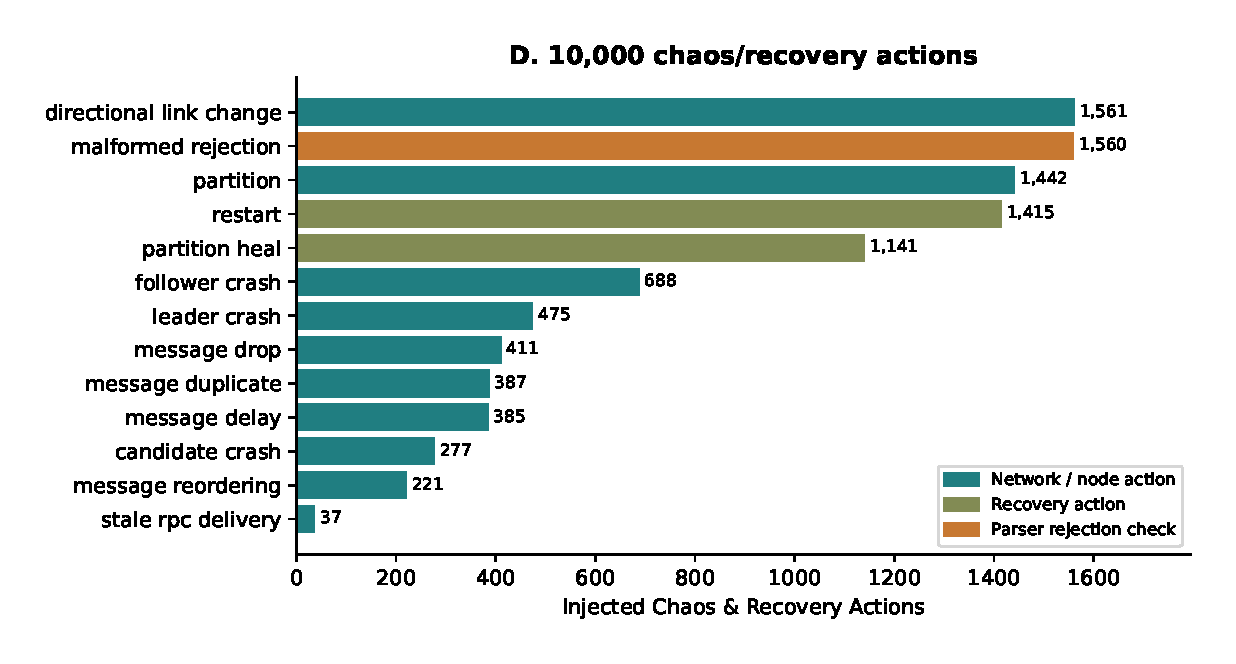
\includegraphics[width=.95\linewidth]{figures/chaos_summary.pdf}
\caption{Injected chaos and recovery actions, including parser checks.
Ordinary ticks are excluded; colors distinguish the action classes.}
\label{fig:chaos}
\end{figure}

Across the twenty runs, the simulator executed \SimulationSeconds{}\,s of
virtual cluster time in \CampaignWallSeconds{}\,s of wall-clock time on Windows
11 with Python 3.12.14. No monitored safety invariant failed in \CheckCount{}
property-group checks, and all twenty final recovery phases converged.
Stale RPC delivery occurred only 37 times because it requires a queued packet
from an earlier term whose destination is alive and reachable. Reordering
occurred 221 times because its selector branch requires at least two queued
packets; link changes and parser checks have less restrictive preconditions.
Restarts and healing account for 2,556 actions, and malformed-input rejections
for another 1,560.

\subsection{E: localhost TCP measurement}
\TCPFindings{}

\section{Limitations}
RaftLight implements leader election and log replication for fixed three- or
five-node clusters with trusted peers. It omits log compaction, snapshots,
membership changes, linearizable read-index or lease reads, and client-session
deduplication.

Each durable update rewrites and synchronizes a full JSON snapshot on the
\texttt{asyncio} event loop. With bounded entry sizes, serialization and write
volume grow as $O(|L|)$ with log length; a slow \texttt{fsync} also delays timers
and peer handling. An append-only write-ahead log with periodic snapshots would
reduce repeated writes, at the cost of more complex recovery and compaction.
Keeping \texttt{storage.py} synchronous lets \texttt{Node} enforce the
persist-before-send invariant directly inside synchronous state transitions
without coloring the consensus core with \texttt{async/await}; a production
runtime would instead emit persistence requests as explicit Sans-I/O output
effects flushed on a background worker before releasing dependent outbound RPCs.

Deterministic scheduling makes partitions, crashes and reordering repeatable
throughout the \FaultCount{}-action campaign. The latency experiments use
independent 1--10\,ms in-memory delays, excluding physical congestion, disk
contention and operating-system scheduling. Campaign reordering may release a
packet before its sampled delivery time; the latency model does not use that
adversarial action.

Historical checks and five mutation witnesses catch failures in executable
traces, but cannot prove safety across every schedule. The monitor itself may
contain bugs; formal verification would require a separate model and
specification. Progress needs a communicating majority and timing conditions
compatible with the election timeout, since fully asynchronous crash-fault
consensus has no unconditional termination guarantee~\cite{flp}.

\section{Conclusion}
RaftLight runs the same durable election and replication rules in asynchronous
TCP nodes and deterministic simulations. Targeted, generated, storage and
real-transport tests complement the \FaultCount{}-event campaign. The experiments
found no monitored safety violations, while recovery and packet-loss measurements
show how availability depends on stable communication. Saved seeds, traces and
mutant controls provide a reproducible baseline for adding log compaction and
dynamic membership.

\begin{thebibliography}{9}
\bibitem{raft} D. Ongaro and J. Ousterhout, ``In Search of an Understandable
Consensus Algorithm,'' USENIX Annual Technical Conference, pp. 305--319, 2014.
Extended version: \url{https://raft.github.io/raft.pdf}.
\bibitem{hypothesis} Hypothesis contributors, ``Stateful tests,'' Hypothesis
documentation, accessed 22 October 2026.
\url{https://hypothesis.readthedocs.io/en/latest/stateful.html}.
\bibitem{lamport} L. Lamport, ``The Part-Time Parliament,''
\emph{ACM Transactions on Computer Systems}, vol. 16, no. 2, pp. 133--169, 1998.
\url{https://doi.org/10.1145/279227.279229}.
\bibitem{flp} M. J. Fischer, N. A. Lynch, and M. S. Paterson,
``Impossibility of Distributed Consensus with One Faulty Process,''
\emph{Journal of the ACM}, vol. 32, no. 2, pp. 374--382, 1985.
\url{https://doi.org/10.1145/3149.214121}.
\bibitem{schneider} F. B. Schneider, ``Implementing Fault-Tolerant Services Using
the State Machine Approach: A Tutorial,'' \emph{ACM Computing Surveys},
vol. 22, no. 4, pp. 299--319, 1990.
\url{https://doi.org/10.1145/98163.98167}.
\bibitem{paxoslive} T. D. Chandra, R. Griesemer, and J. Redstone,
``Paxos Made Live: An Engineering Perspective,''
\emph{Proceedings of the 26th ACM Symposium on Principles of Distributed Computing},
pp. 398--407, 2007. \url{https://doi.org/10.1145/1281100.1281103}.
\end{thebibliography}

\clearpage
\appendix
\section{Reproduction and artifact inventory}
Run these commands from the repository root with Python 3.12 or later.
The listing uses Bash/POSIX shell continuation. In PowerShell, join each
continued command onto one line, as shown in the README.
{\small
\begin{verbatim}
python -m venv .venv
# Activate .venv using the command for your shell.
python -m pip install -r requirements.txt
python -m pytest -q
python test_network_hell.py --faults 10000 --seed 20261022 --trials 20
python benchmarks/run_benchmarks.py --trials 100 --writes 5 \
  --election-trials 200 --recovery-trials 20
python tools/run_sensitivity.py
python benchmarks/run_tcp_benchmark.py --writes 100 --seed 42 \
  --data-dir data/tcp-run
\end{verbatim}
}
The TCP benchmark requires a fresh state directory; use \texttt{-{}-data-dir} to
select another directory when repeating it. Localhost ports are selected
automatically.

\begin{itemize}
\item \textbf{Core implementation:} \texttt{raftlight/} contains consensus,
messages, state machine, storage, TCP runtime and simulator;
\texttt{raft.py} provides the node and client commands.
\item \textbf{Verification suite:} \texttt{tests/} covers unit, generated and
real TCP cases; \mbox{\texttt{test\_network\_hell.py}} runs the chaos campaign;
\mbox{\texttt{tools/run\_sensitivity.py}} runs the five mutant witnesses.
\item \textbf{Experimental artifacts:} \texttt{benchmarks/} produces measurements
and plots from the JSON observations in \texttt{results/}, which also contains
the twenty chaos traces and real TCP timings. The four empirical PDF/PNG pairs
(Figures~2--5) are in \texttt{report/figures/}; Figure~1 is the TikZ architecture
diagram. The README gives cluster and report build commands.
\end{itemize}

\section{Representative trace}
The following shortened trace is from the saved three-node run with seed
20261022. Times are simulated seconds; writes and ordinary scheduling are not
counted as disasters. The full trace preserves the intervening events.
{\small
\begin{verbatim}
0.500000  disable directional link 3 -> 2
0.500000  submit SET key0 20261022:0 to node 3
0.535777  disable directional link 1 -> 3
0.547835  heal network
0.563545  crash node 3
0.574257  submit command: no known leader
0.624681  restart node 3 from durable term/vote/log
0.665745  disable directional link 2 -> 3
0.713152  reject malformed RequestVote (negative term)
0.817762  heal network
0.852036  duplicate queued packet 56
0.887862  partition [3,2] | [1]
0.919785  crash node 3
0.953349  crash node 2
1.017109  crash node 1
\end{verbatim}
}
When the trace leaves no quorum available, progress stops while safety checks
continue. Restarted
servers resume as followers with empty volatile application state and reconstruct
their committed state through subsequent valid replication.

\clearpage
\section{Sampling uncertainty}
For each loss rate, the bootstrap draws \LatencyTrials{} observed seed blocks
with replacement. Every selected block carries its \WritesPerTrial{} offered
outcomes, including timeouts and no-leader attempts. The resample's successful
latencies supply its p50, p95 and p99 estimates; successful attempts divided by
all offered attempts supply availability. Resampling whole seed blocks preserves
dependence between sequential operations sharing one simulated cluster.

The \BootstrapReplicates{} replicates use NumPy's seeded generator with seed
$40000+\text{loss percentage}$. The 2.5th and 97.5th percentiles across replicates
form the pointwise intervals below. Figure~\ref{fig:latency} shades the p95
latency interval; the raw and summary JSON files preserve the observations,
bootstrap seed and sample counts for every loss rate.

At high loss, fewer successful writes leave the p99 less precisely estimated;
the intervals describe the observed seed blocks and retain the three-second
deadline.
\begin{table}[H]\centering\small
\caption{Seed-block bootstrap 95\% confidence intervals
(\BootstrapReplicates{} replicates). Latency units are simulated ms;
availability is a percentage of all \OfferedPerLoss{} offered attempts.
Successful sample sizes appear in Table~\ref{tab:loss}.}
\label{tab:bootstrap}
\begin{tabular}{rrrrr}\toprule
Loss (\%) & p50 interval & p95 interval & p99 interval & Availability interval\\\midrule
\UncertaintyRows
\bottomrule\end{tabular}
\end{table}
\end{document}
